\subsection{Classification trees}

The following section has the purpose to use tree-based classification methods to find a model which will predict if an NBA's rookie career will be longer than five years.

We started to analyze the data through classification trees using the \textit{gini} minimization function. The result is a complex tree which is difficult to read (144 terminal nodes).

To understand whether it was better to use a simpler tree or not, we performed cross-validation using different levels of tree size and evaluated the impact on the test error.

\Fig~\ref{fig:tree_cv_plot} shows the trends of the deviance and the penalization factor \textit{k} for different values of tree size as determined by cross-validation. In \Fig~\ref{fig:trees_size} are shown the obtained trees with different sizes.

\begin{figure}[H]
	\centering
	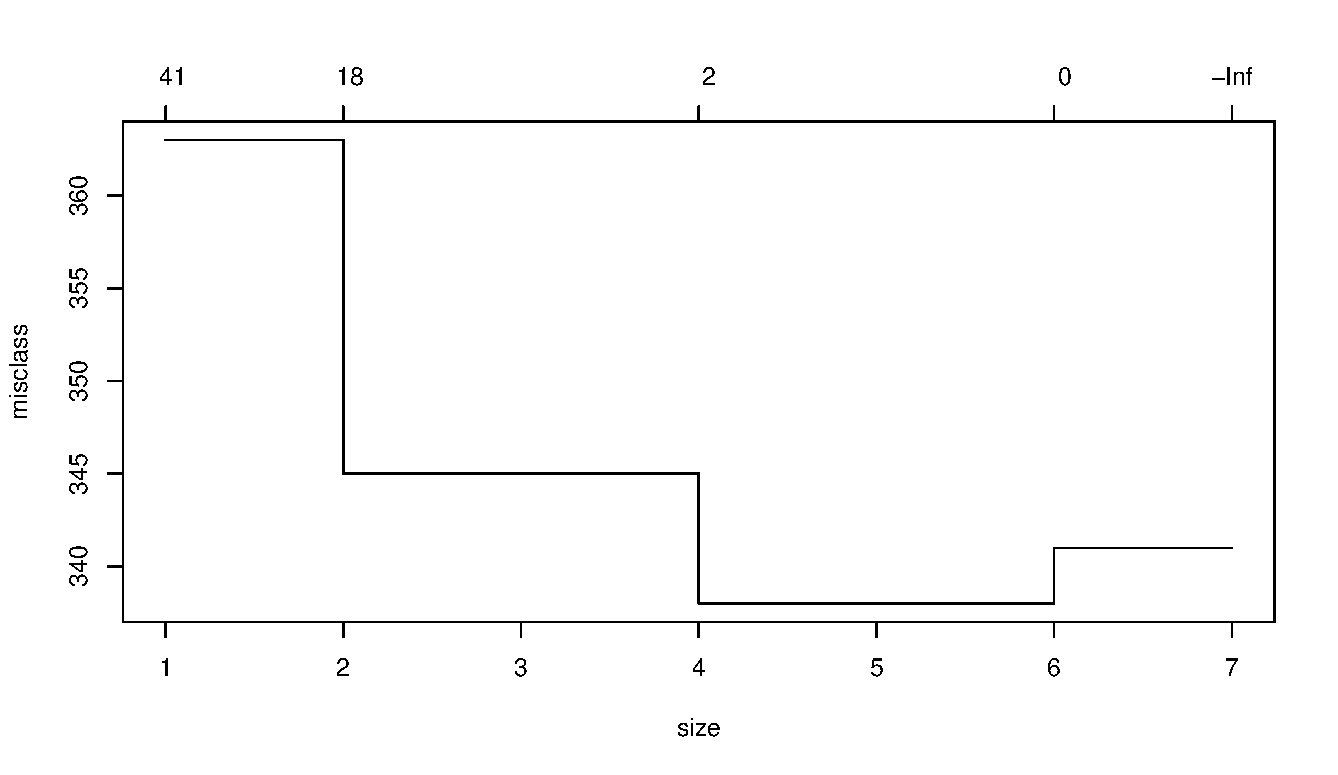
\includegraphics[width=0.5\linewidth]{ImageFiles/Classification/Trees/tree_cv_plot.pdf}
	\caption{Size (bottom), deviance (left), k (top).}
	\label{fig:tree_cv_plot}
\end{figure}

\begin{figure}[H]
	\centering
	\begin{subfigure}{.6\textwidth}
		\centering
		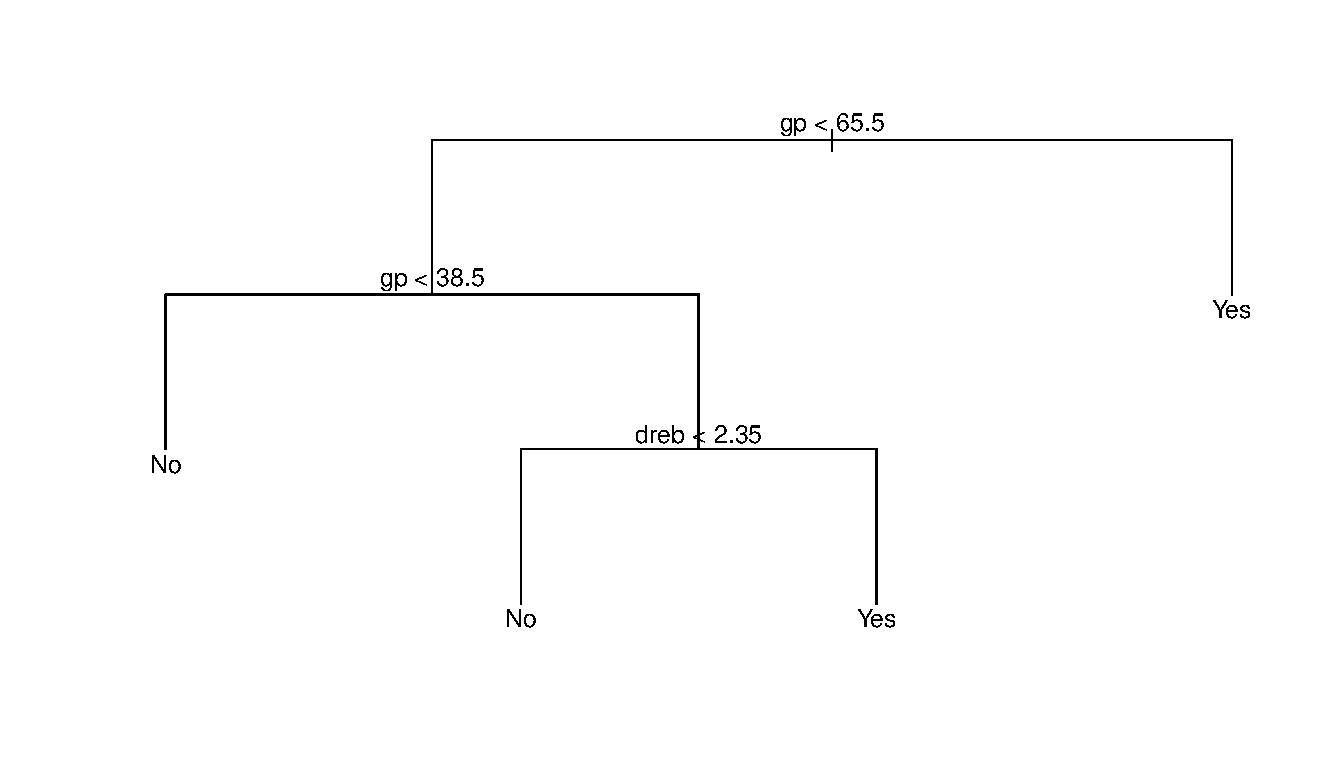
\includegraphics[width=0.5\linewidth]{ImageFiles/Classification/Trees/tree_size_4.pdf}
		\caption{}
		\label{fig:tree_size_4}
	\end{subfigure}%
	\begin{subfigure}{.6\textwidth}
		\centering
		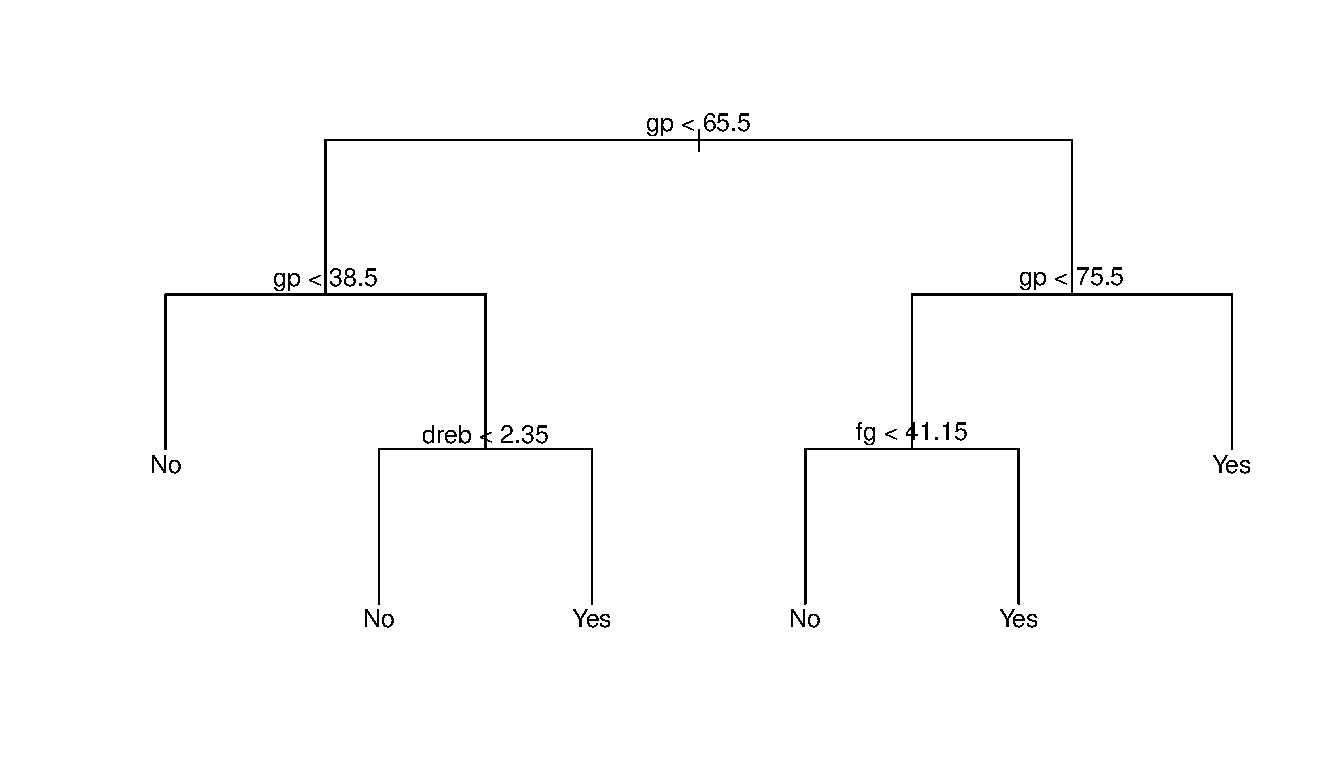
\includegraphics[width=0.6\linewidth]{ImageFiles/Classification/Trees/tree_size_6.pdf}
		\caption{}
		\label{fig:tree_size_6}
	\end{subfigure}
	\begin{subfigure}{.6\textwidth}
		\centering
		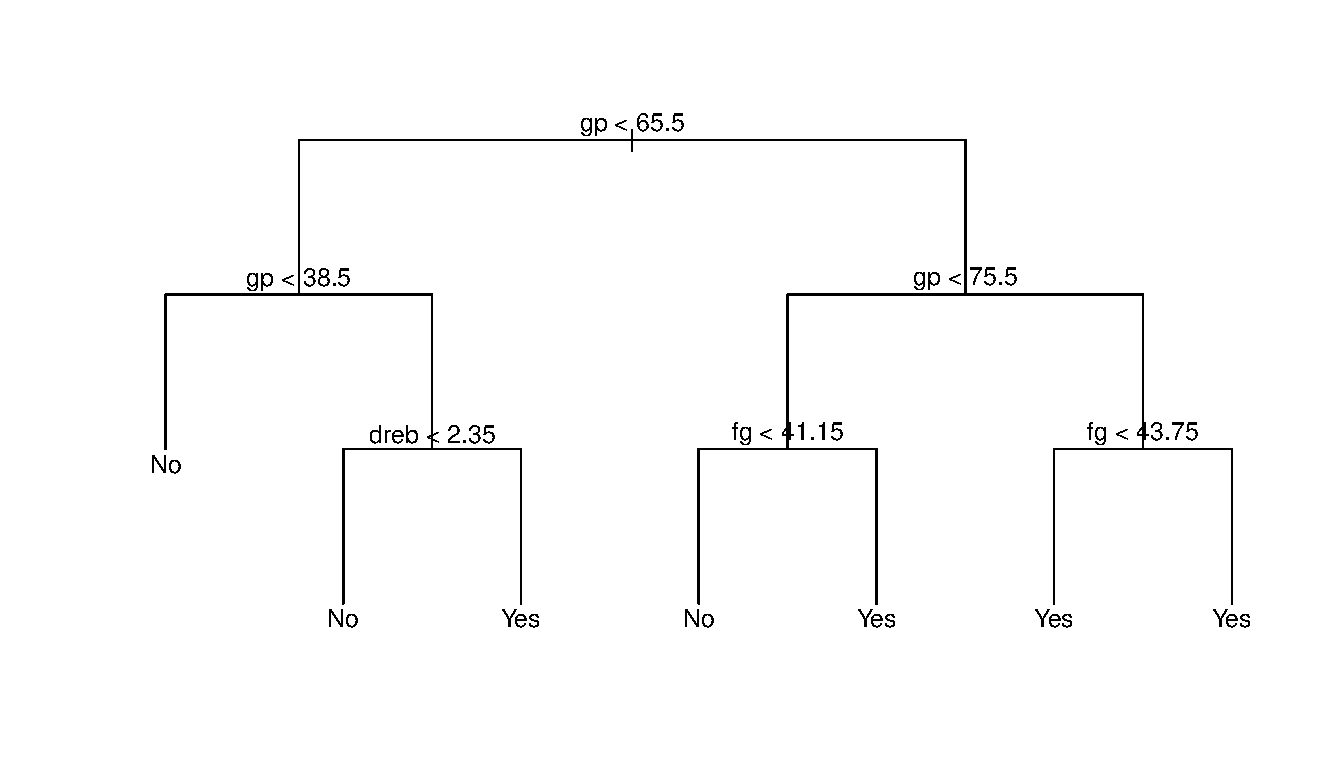
\includegraphics[width=0.5\linewidth]{ImageFiles/Classification/Trees/tree_size_7.pdf}
		\caption{}
		\label{fig:tree_size_7}
	\end{subfigure}%
	\begin{subfigure}{.6\textwidth}
		\centering
		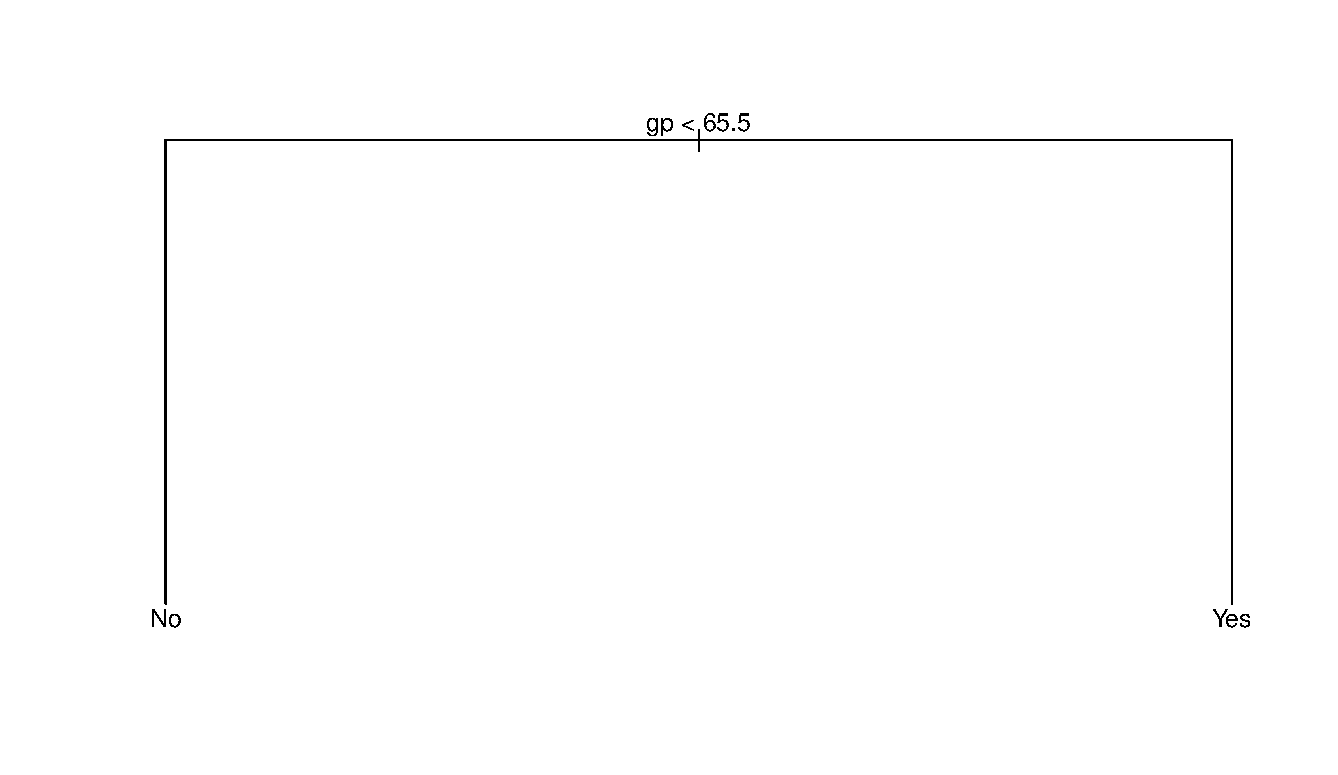
\includegraphics[width=0.6\linewidth]{ImageFiles/Classification/Trees/tree_size_2.pdf}
		\caption{}
		\label{fig:tree_size_2}
	\end{subfigure}
	\caption{Trees with various sizes.}
	\label{fig:trees_size}
\end{figure}

After the evaluation of the misclassification error rate on both train and test dataset, we concluded that the best model is the one with $size = 4$.

\todo{QUALI RISULTATI RIPROTARE?}
Residual Mean Deviance and Misclassification Error rate (train) -> test error rate
\begin{itemize}
	\item 4: 1.153 \& 0.3038 -> 0.3000
	\item 6: 1.114 \& 0.2996 -> 0.33125
	\item 7: 1.098 \& 0.2996 -> 0.33125
	\item 2: 1.200 \& 0.3424 -> 0.33125
\end{itemize}

However, all the trees do the first split on the variable ``GP'', suggesting that it is the most important variable.
